%
% Beamer slides for the thesis.
%
% NOTE: the "Padova" theme is needed to compile this file.
%       It can be found here: http://www.math.unipd.it/~burattin/other/tema-latex-beamer-padova/files/beamer_padova-0.3.zip
%
\pdfminorversion=4
\documentclass{beamer}
\usetheme{Padova}
% Include the following packages:
\usepackage{mathtools}
\usepackage{pgfpages}
\pgfpagesuselayout{resize to}[a4paper,landscape,border shrink=5mm]

\title{Studio dell'efficienza di oscillatori LC integrati per impulsatori
	Ultra-Wideband}
\author{Laureando: Paolo Scaramuzza \\ Relatore: Andrea Neviani}
\date{29 Settembre 2014}

\begin{document}
%
%% title
\begin{frame}
\maketitle
\end{frame}
%
%% outline
\begin{frame}
\frametitle{Contenuti}
\begin{enumerate}
	\item Motivazione
	\vfill % bigger space between items
	\item Tipologie di oscillatore
	\vfill
	\item Modello teorico
	\vfill
	\item Simulazioni
	\vfill
	\item Conclusioni e sviluppi futuri
	\vfill
\end{enumerate}
\end{frame}
%
%% UWB-IR description & application
\begin{frame}
\frametitle{La radio a impulsi UWB}
\begin{itemize}
	\item Trasmette i dati sotto forma di impulsi
	\vfill
	\item Impieghi:
	\begin{itemize}
		\item Trasmissione a corto raggio
		\item Localizzazione di precisione
	\end{itemize}
	\vfill
	\item Facilmente integrabile in tecnologia CMOS
	\vfill
	\item Pu\`o operare tramite \emph{energy harvesting}
	\vfill
\end{itemize}
\end{frame}
%
%% LC cross-coupled oscillator topology
\begin{frame}
\frametitle{L'oscillatore LC \emph{cross-coupled}}
\begin{columns}
	\column[t]{0.5\textwidth}
	\begin{flushleft}
      \begin{figure}
      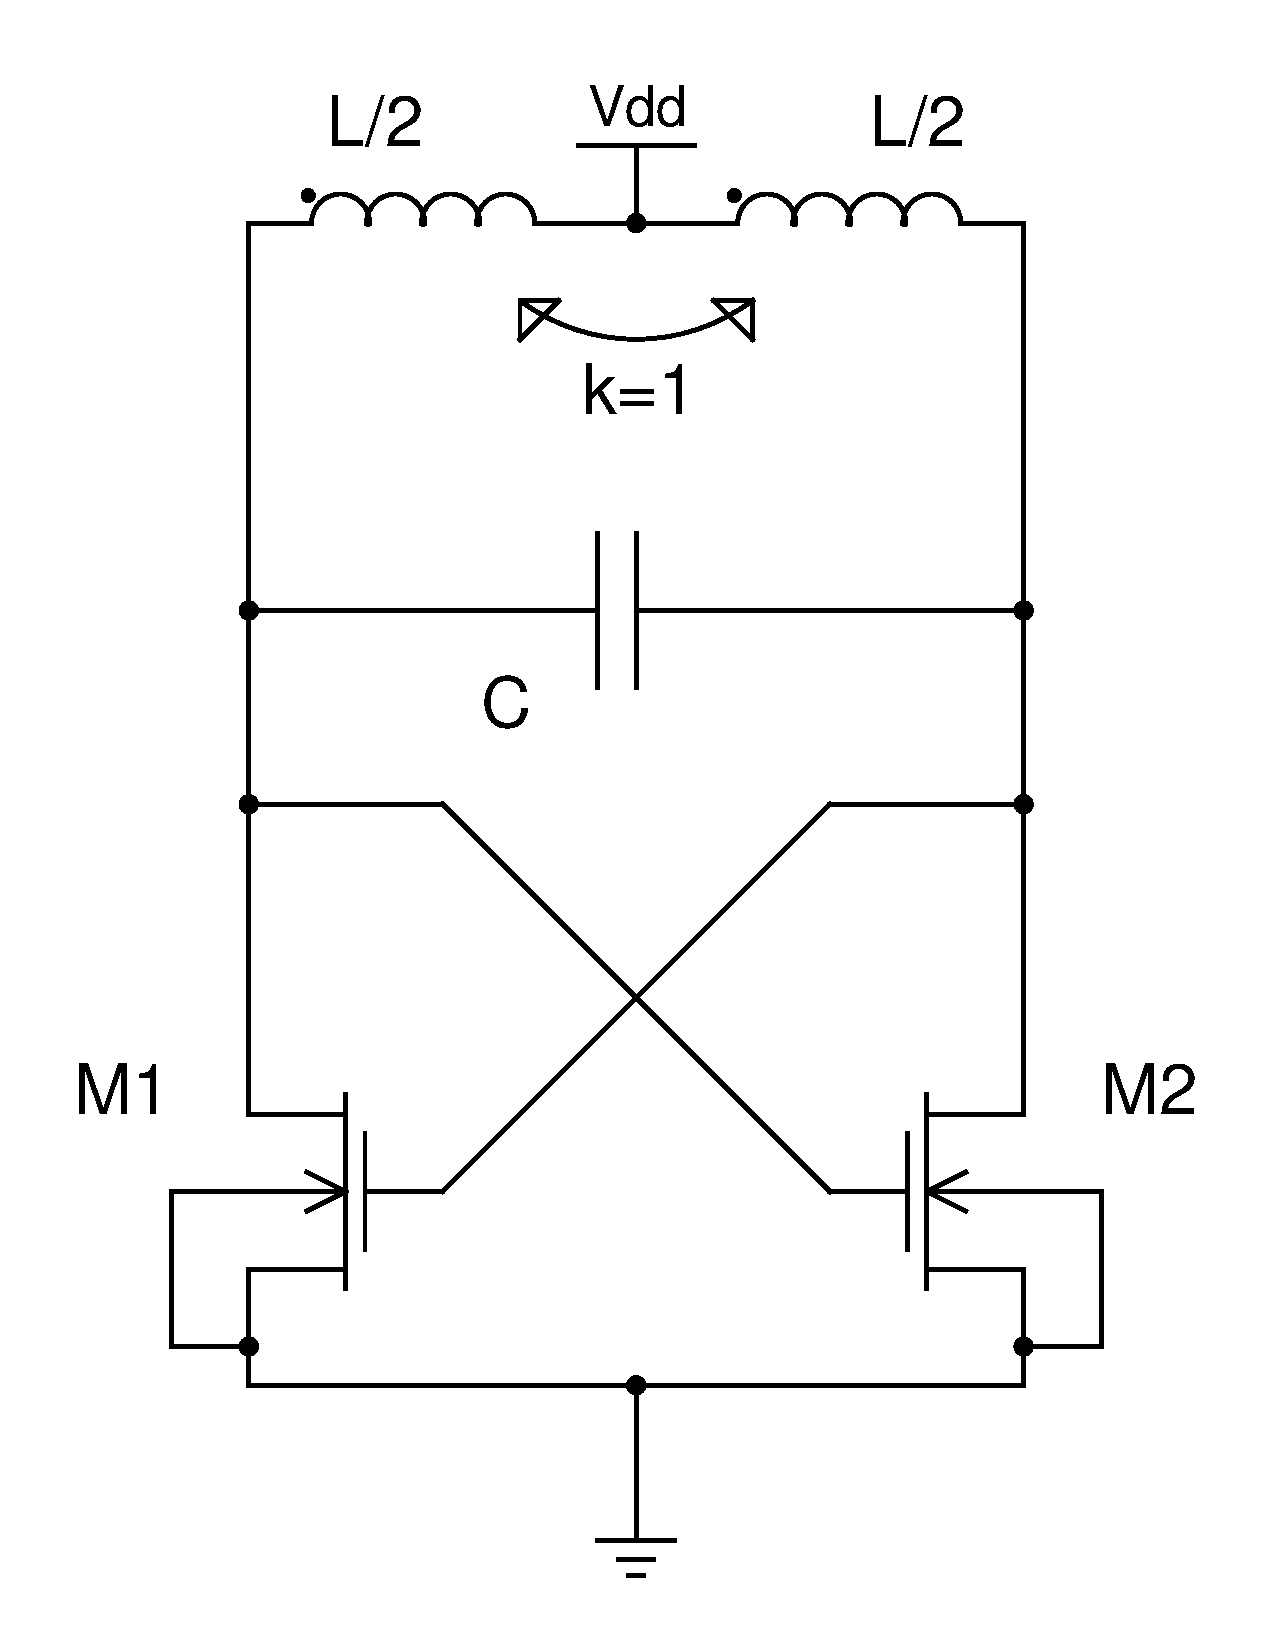
\includegraphics[width=\textwidth]{images/LCosc.pdf}
      \end{figure}
	\end{flushleft}
	
	\column[t]{0.5\textwidth}
	\begin{itemize}
		\item Basso numero di componenti attivi
		\bigskip
		\item Rumore di fase inferiore ad altre soluzioni
		\bigskip
		\item Frequenza di oscillazione:\\
			\smallskip
			{\large $ f_{osc} = \frac{1}{2\pi\sqrt{LC}}$}
	\end{itemize}
\end{columns}
\end{frame}
%
%% Oscillator types
\begin{frame}
\frametitle{Tipologie di oscillatore considerate}
\begin{columns}
	\column[t]{0.5\textwidth}
	\begin{flushleft}
      \begin{figure}
      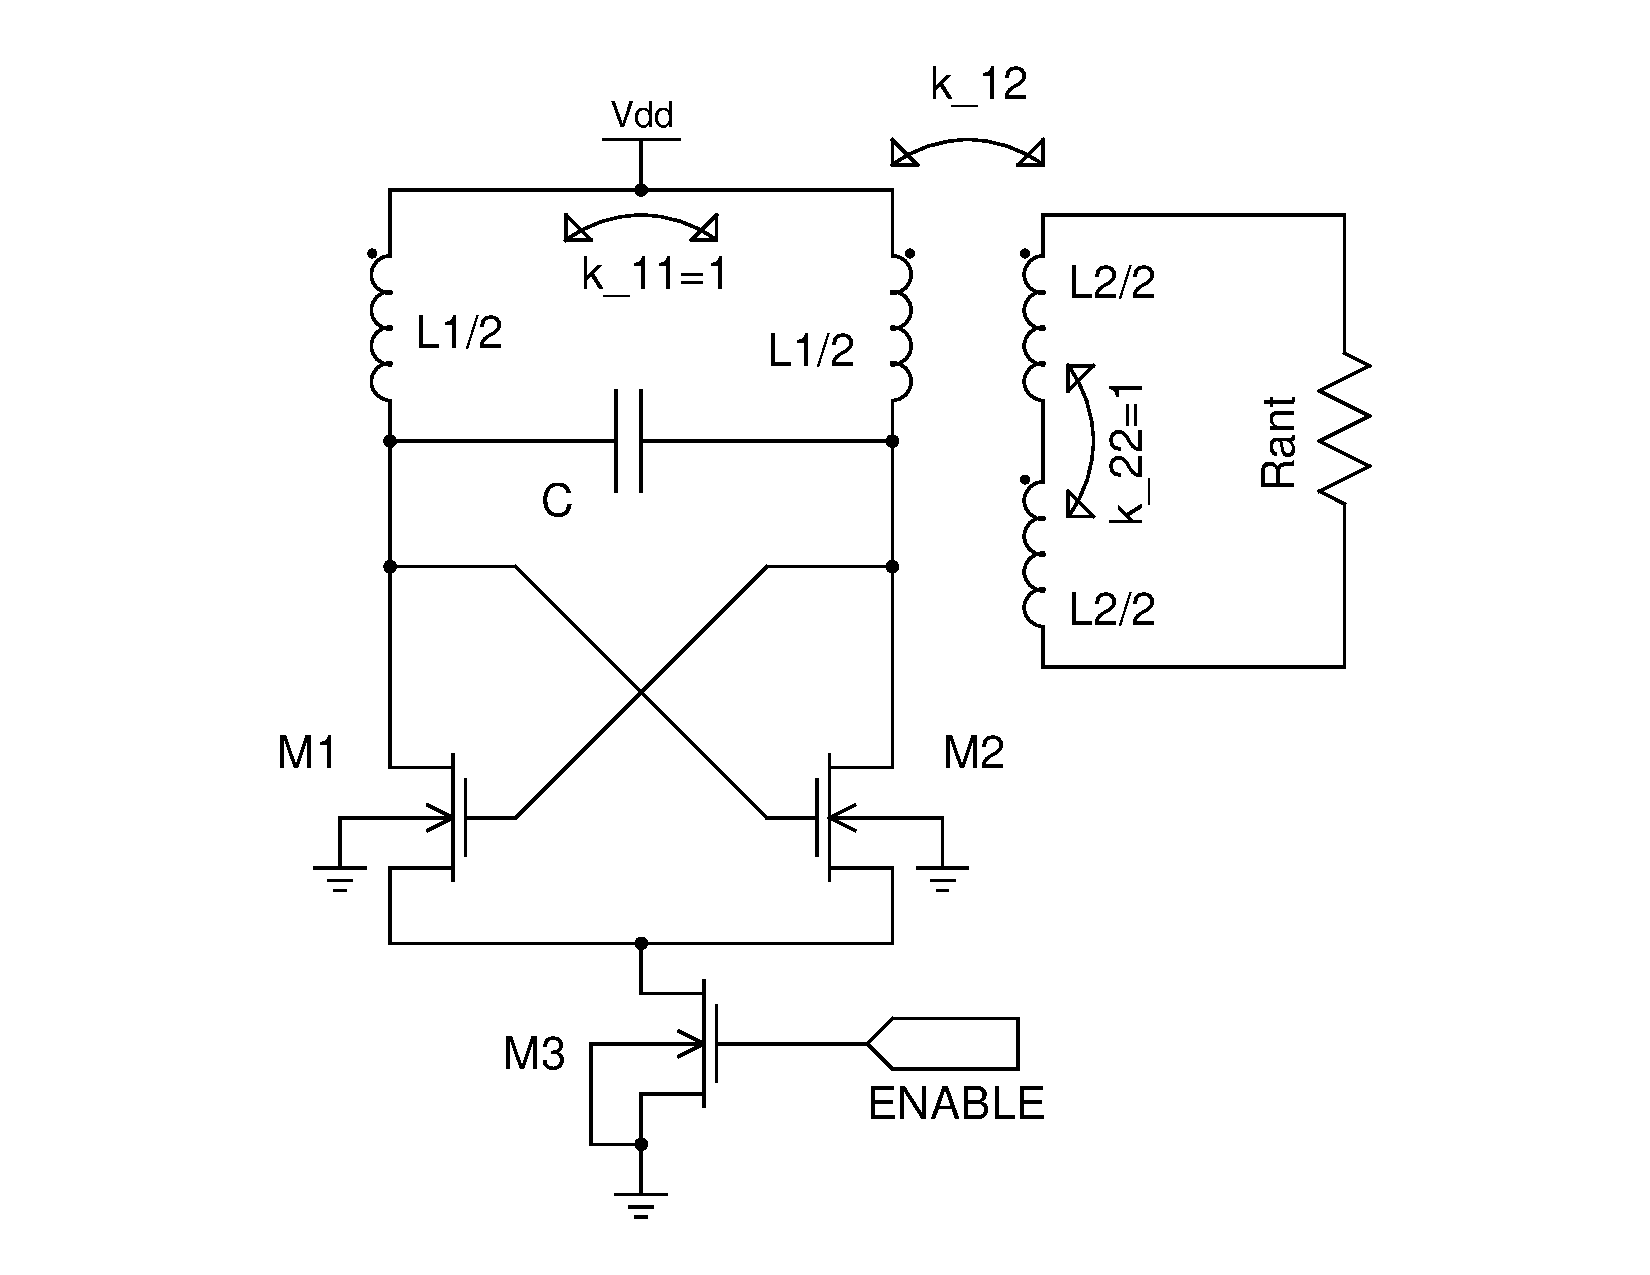
\includegraphics[width=\textwidth]{images/tipo1.pdf}
      \end{figure}
      \end{flushleft}
	\center{Oscillatore "Tipo 1"}

	\column[t]{0.5\textwidth}
      \begin{flushright}
      \begin{figure}
      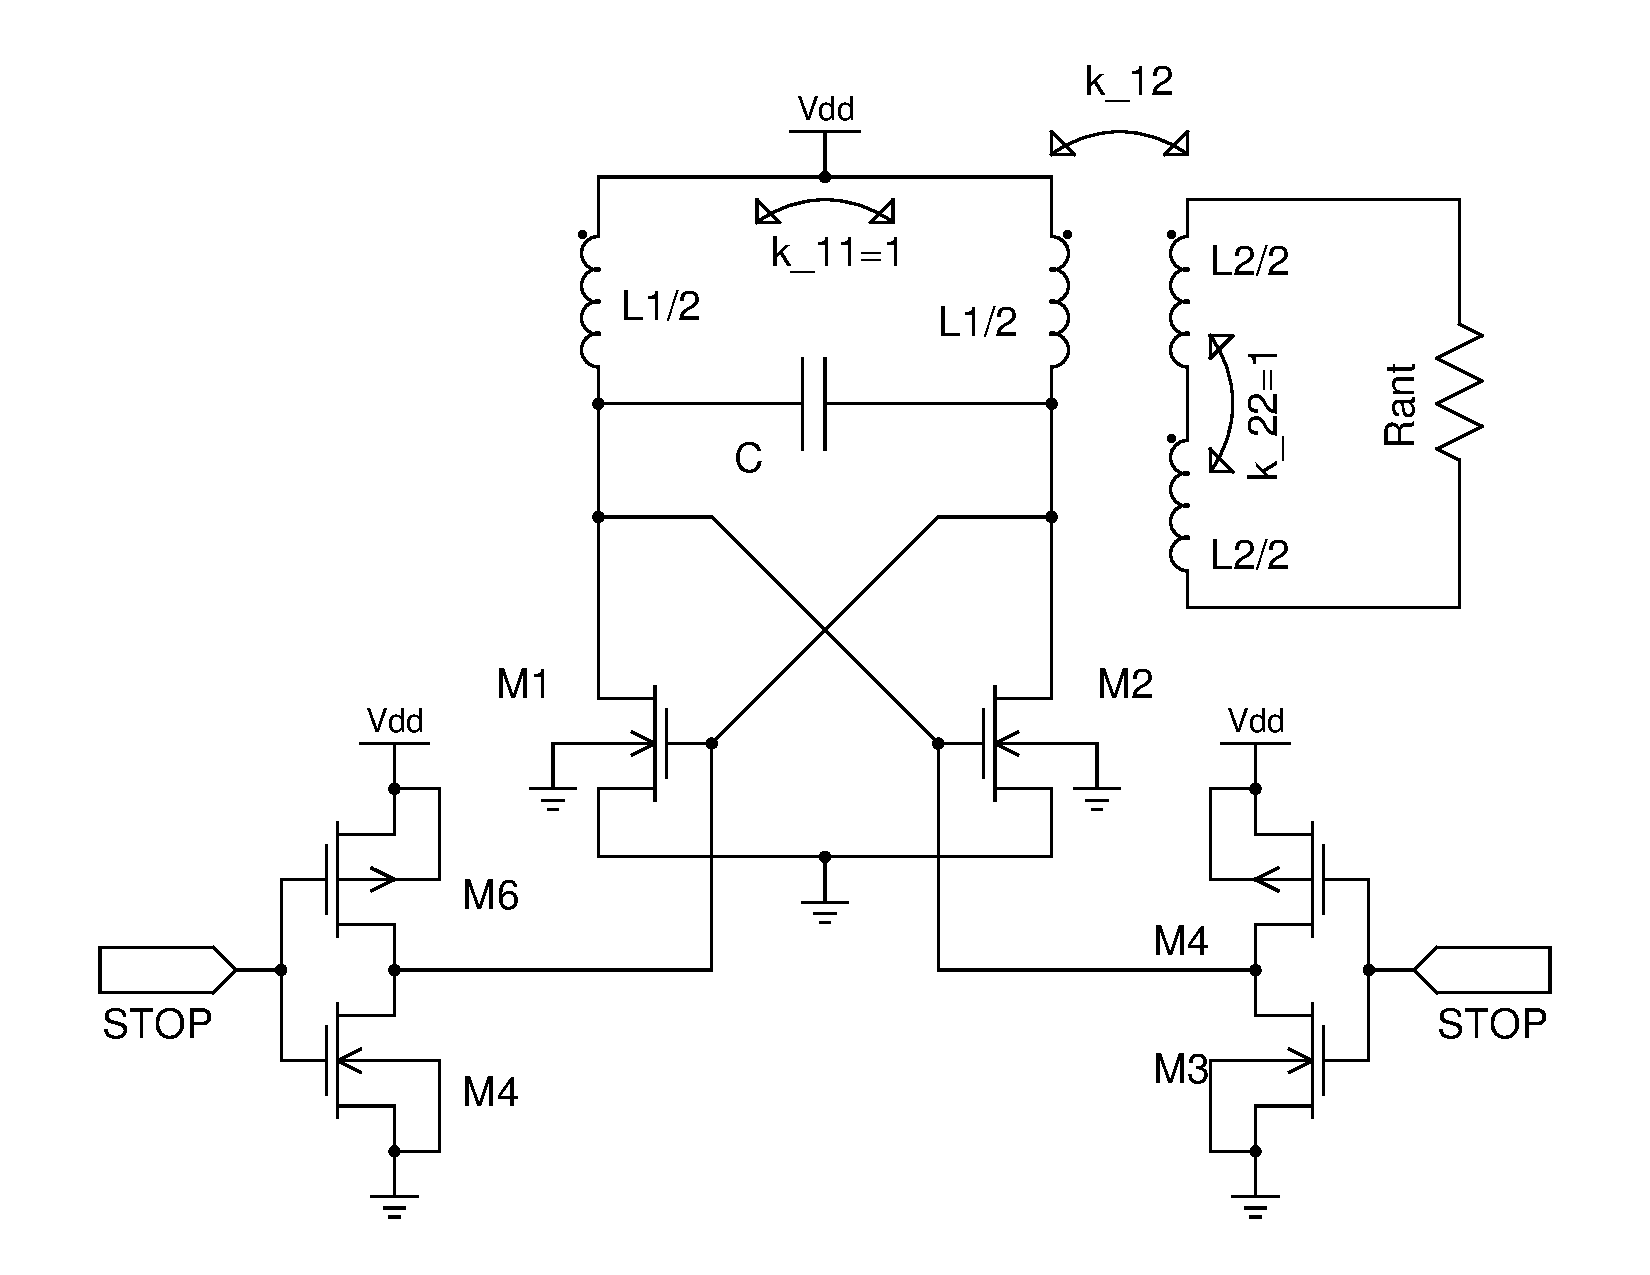
\includegraphics[width=\textwidth]{images/tipo2.pdf}
      \end{figure}
      \end{flushright}
	\center{Oscillatore "Tipo 2"}
\end{columns}
\end{frame}
%
%% Transformer model (maybe join with the theoretical model)
\begin{frame}
\frametitle{Modello del trasformatore}
\begin{figure}
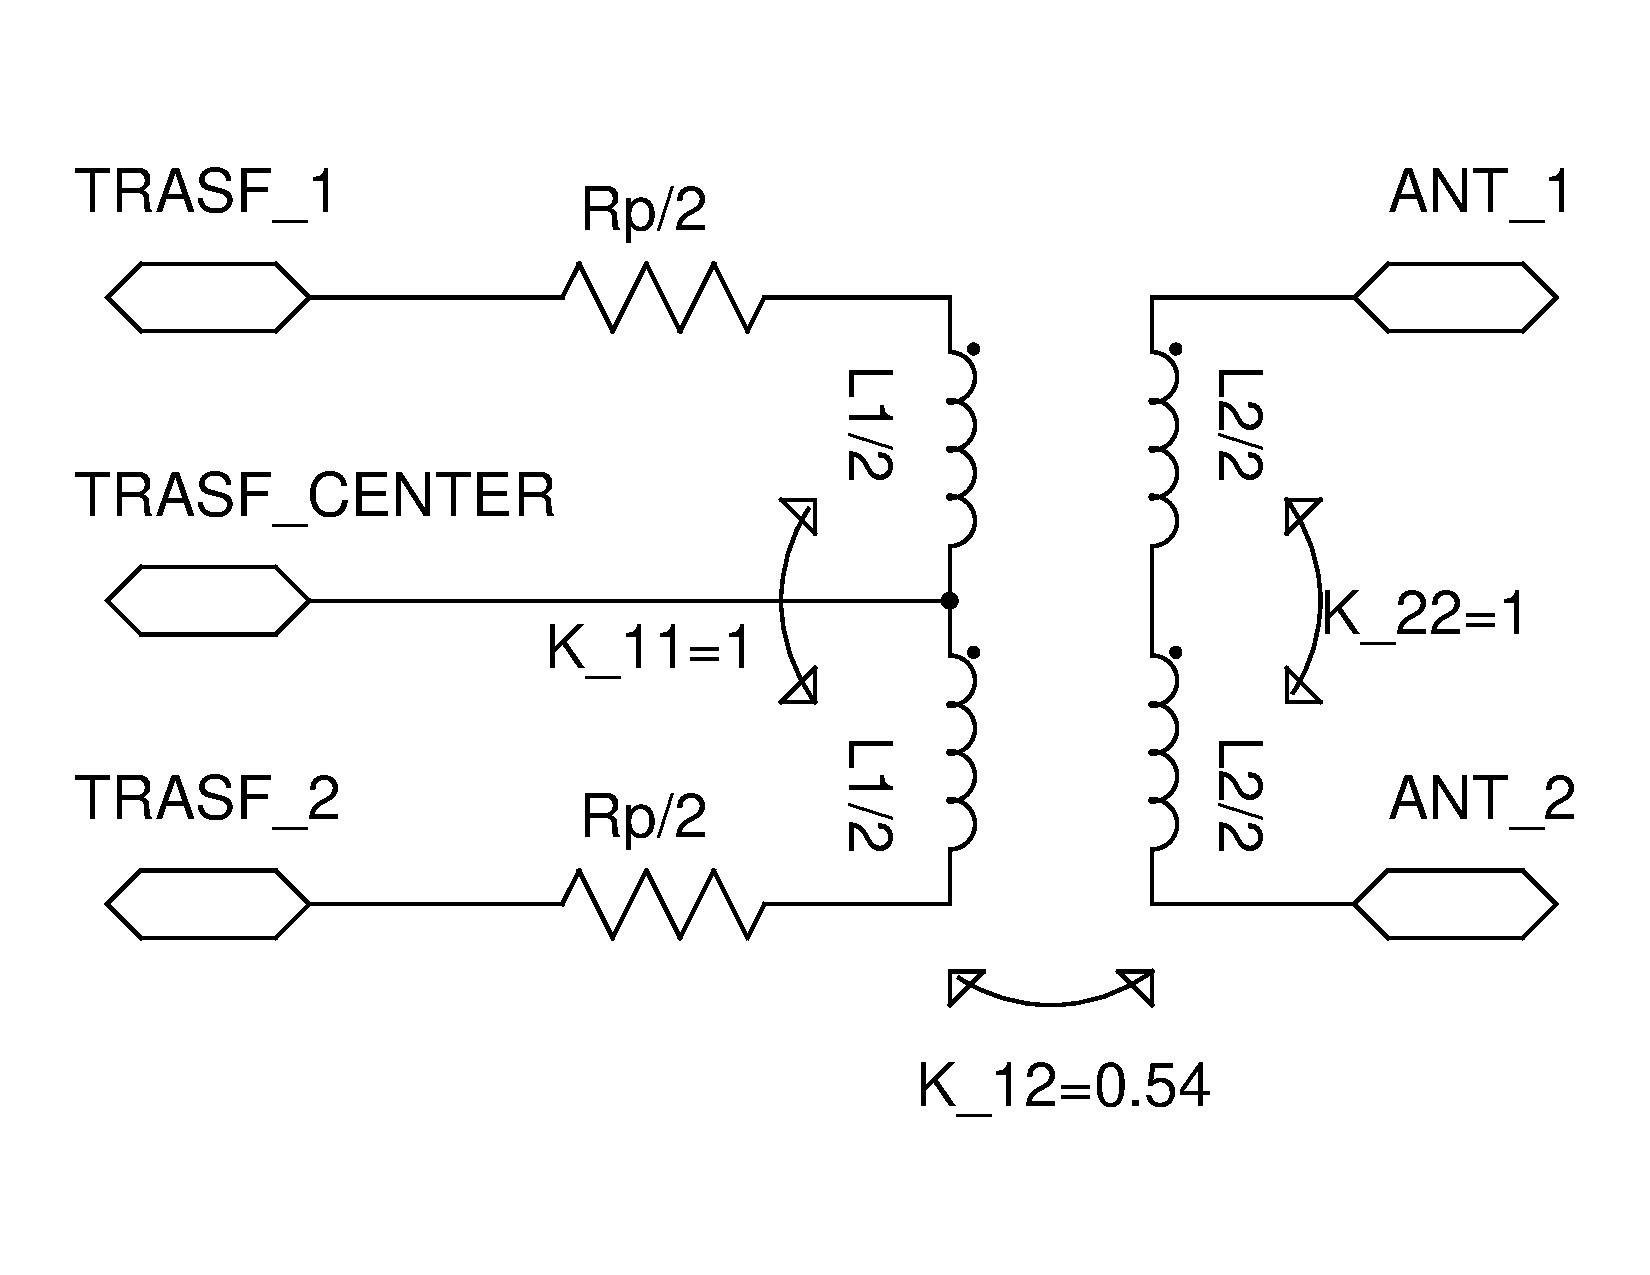
\includegraphics[height=0.4\textheight]{images/trasf_model.pdf}
\end{figure}
\begin{itemize}
	\item Modello con resistenza in serie al primario
	\item Si trascurano le capacit\`a e le induttanze parassite.
	\item $R_s=\omega_0 \frac{L_1}{Q}\, ,\;\; Q=25$
\end{itemize}
\end{frame}
%
%% Theorical model
\begin{frame}
\frametitle{Modello teorico}
\begin{columns}
	\column[t]{0.5\textwidth}
	I MOSFET producono un'onda sinusoidale di ampiezza $2V_{DD}$.
	\begin{figure}
	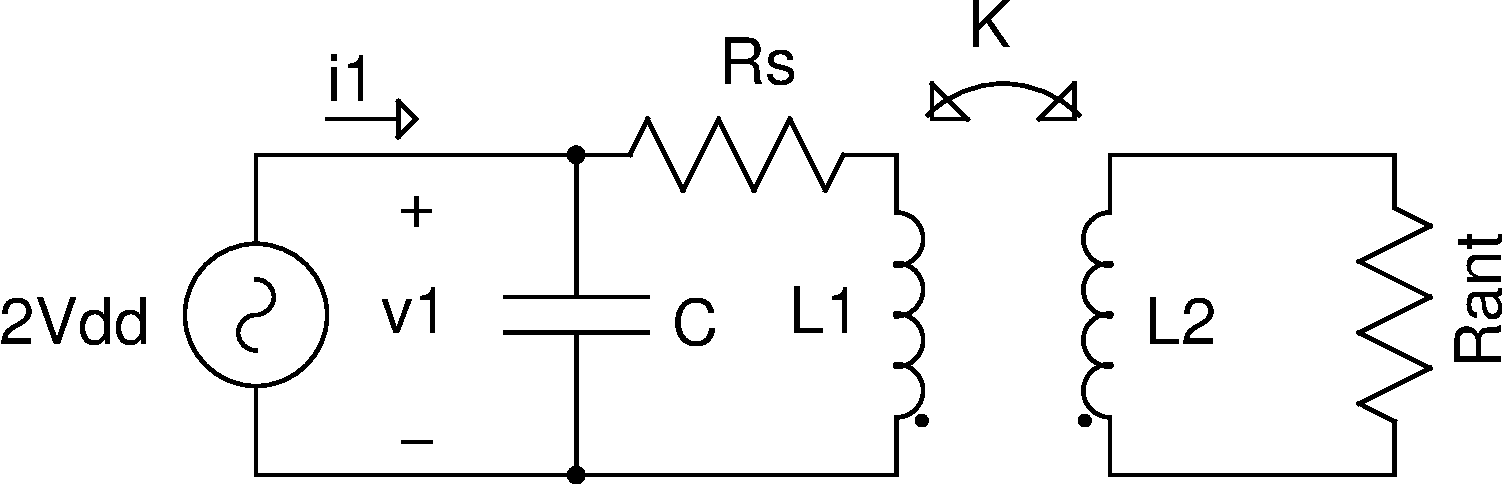
\includegraphics[width=\textwidth]{images/cir_model.pdf}
	\end{figure}
	Applicando le trasformazioni serie-parallelo:
	\begin{figure}
	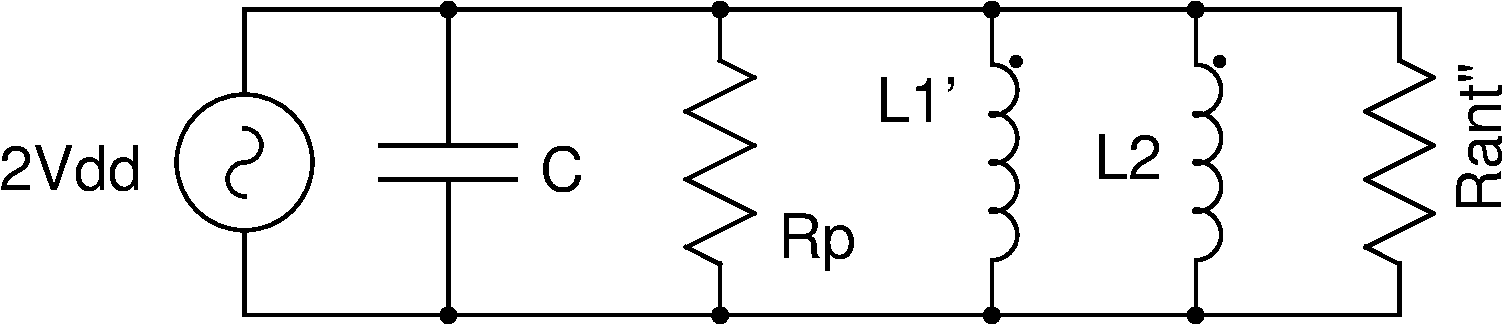
\includegraphics[width=\textwidth]{images/cir_model3.pdf}
	\end{figure}

	\column[t]{0.5\textwidth}
	Induttanze a capacit\`a sono in risonanza. Si ottiene un partitore
	resistivo.
	\medskip
	$$ \eta_t = \frac{aL_2^2}{R_{ant}^2 + ( a + b^2 )^2L_2^2} $$
	$ a = (K\omega_0)^2\frac{R_{ant}}{R_s} $\\
	\smallskip
	$ b = (1 - K^2)\omega_0 $\\
	\medskip
	\center\framebox{$\eta_t \rightarrow 1 \Longleftrightarrow L_1
	\rightarrow 0, L_2 \rightarrow +\infty $}
\end{columns}
\end{frame}
%
%% Simulation results
\begin{frame}
\frametitle{Risultati delle simulazioni}
\vspace{-0.6cm} % correct wrong figure margins
\begin{figure}
\centering
\includegraphics[height=0.8\textheight]{efficienza.pdf}
\end{figure}
\end{frame}
% some more results
\begin{frame}
\begin{columns}
\column[t]{0.75\textwidth}
\begin{figure}
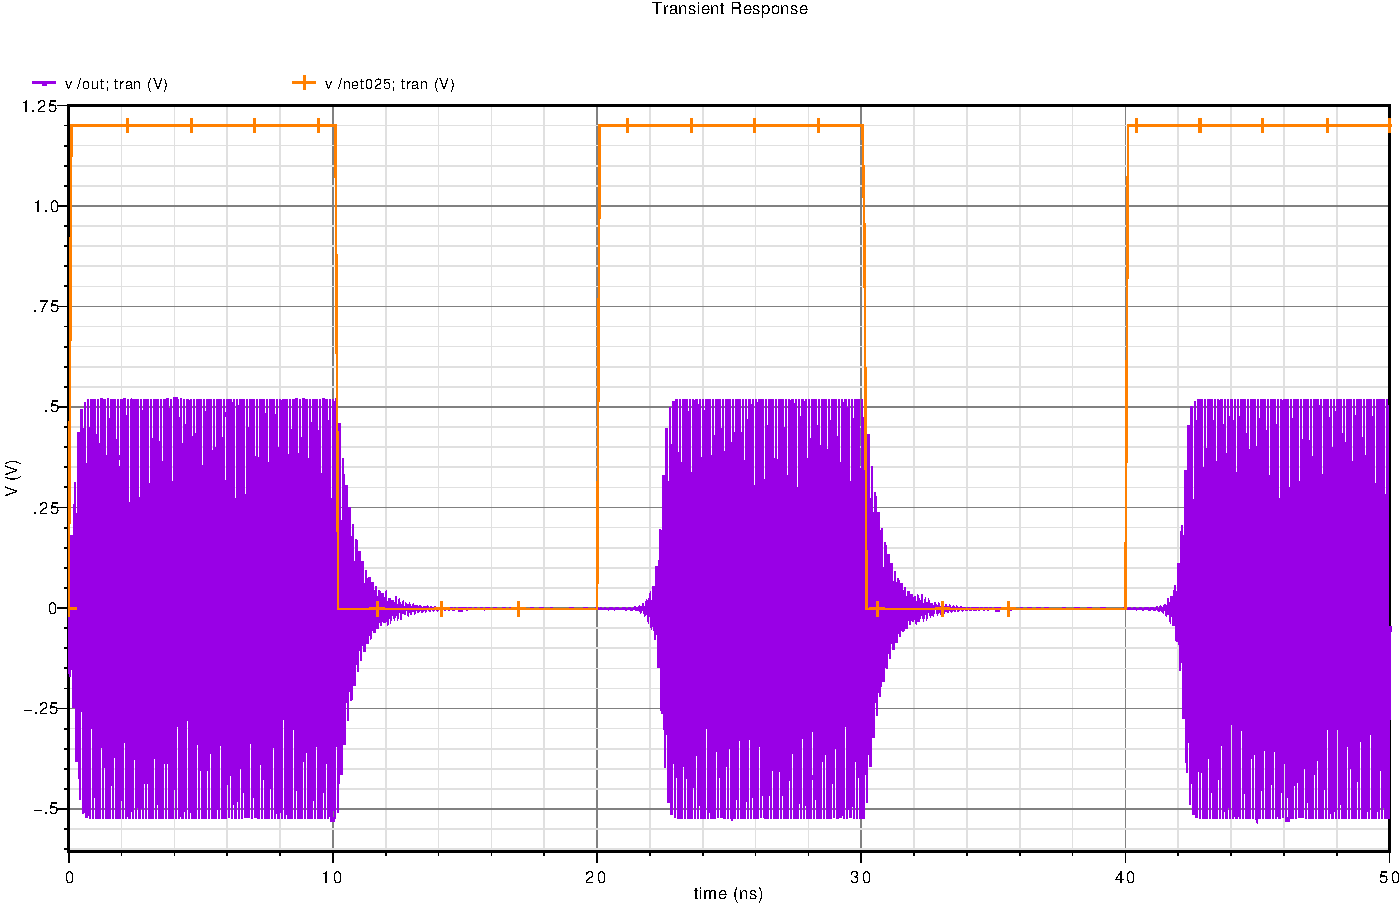
\includegraphics[width=\textwidth]{images/tipo1-impulsato.pdf}
\end{figure}
Oscillatore di Tipo 1, funzionamento impulsato.

\column[t]{0.25\textwidth}
      \vspace{0.5cm}
      \begin{figure}
      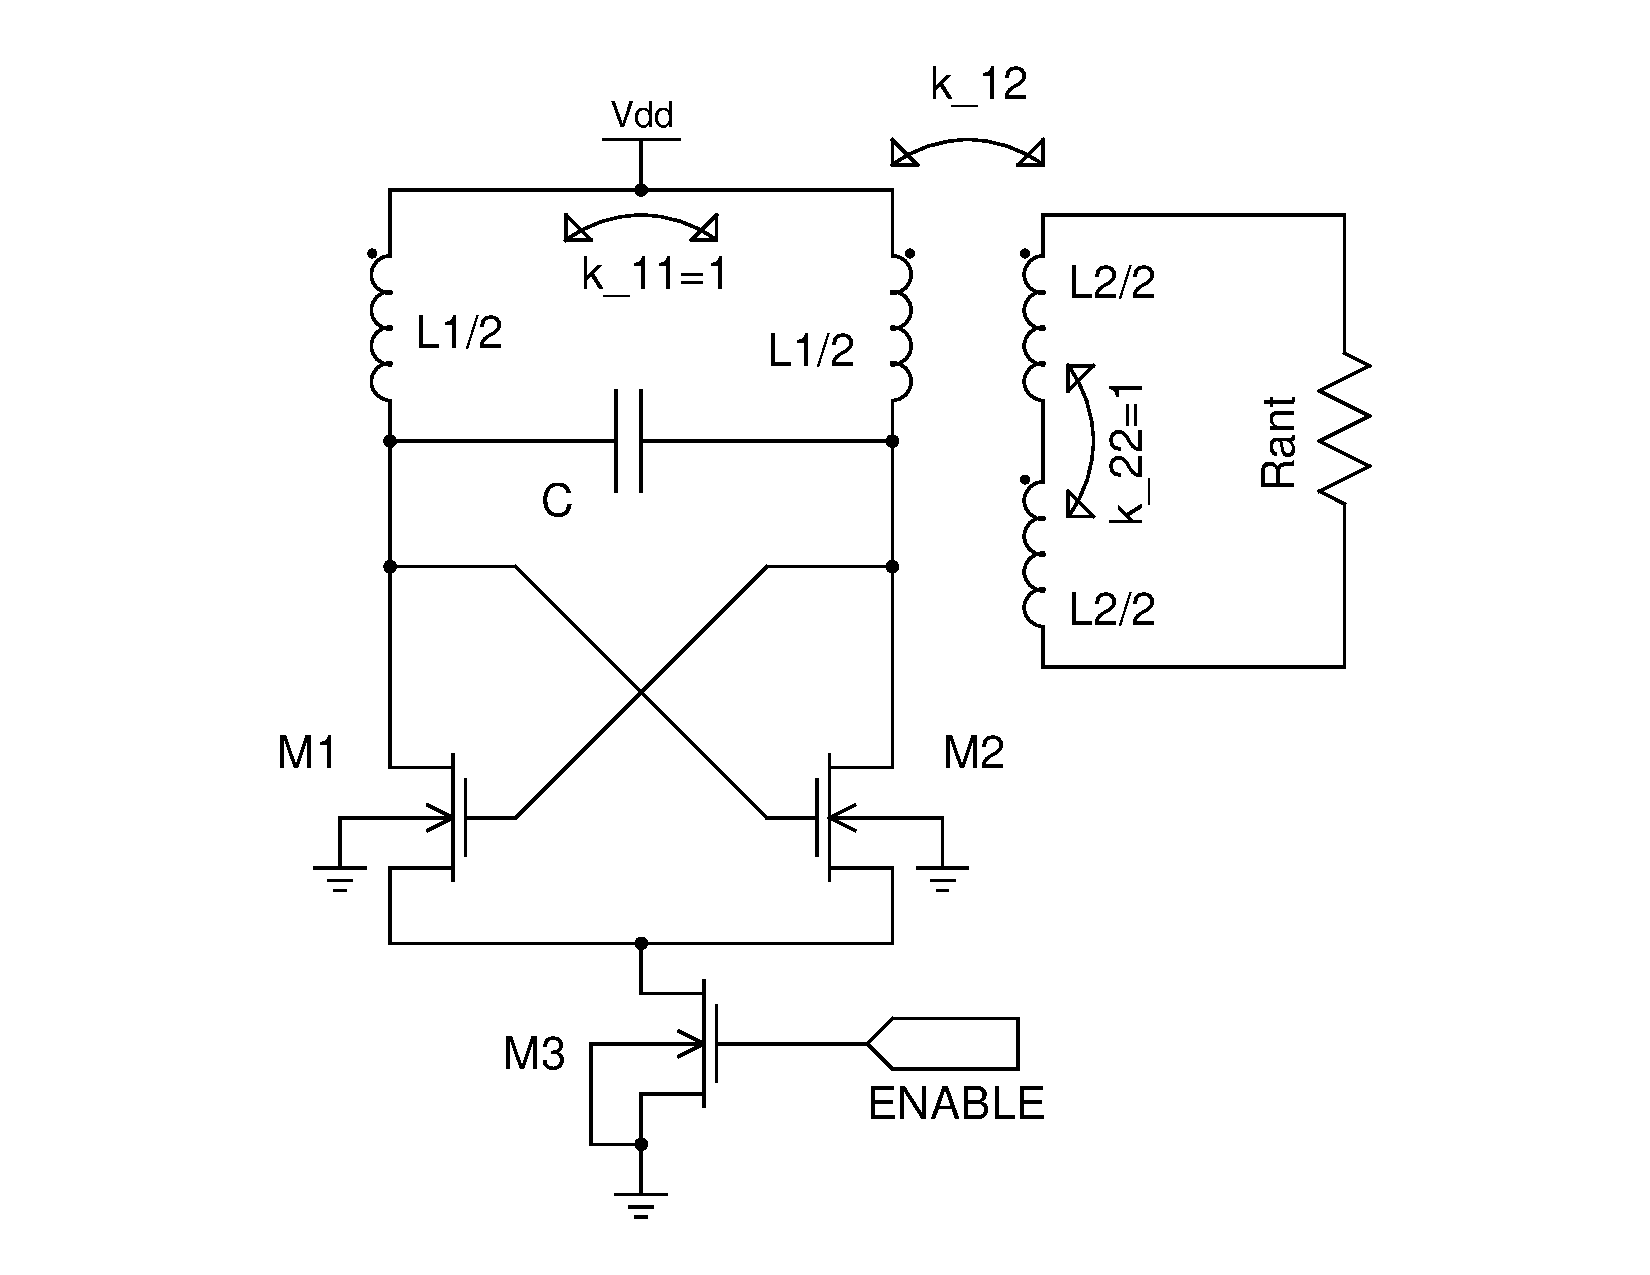
\includegraphics[width=1.5\textwidth]{images/tipo1.pdf}
      \end{figure}
\end{columns}
\end{frame}

\begin{frame}
\begin{columns}
\column[t]{0.75\textwidth}
\begin{figure}
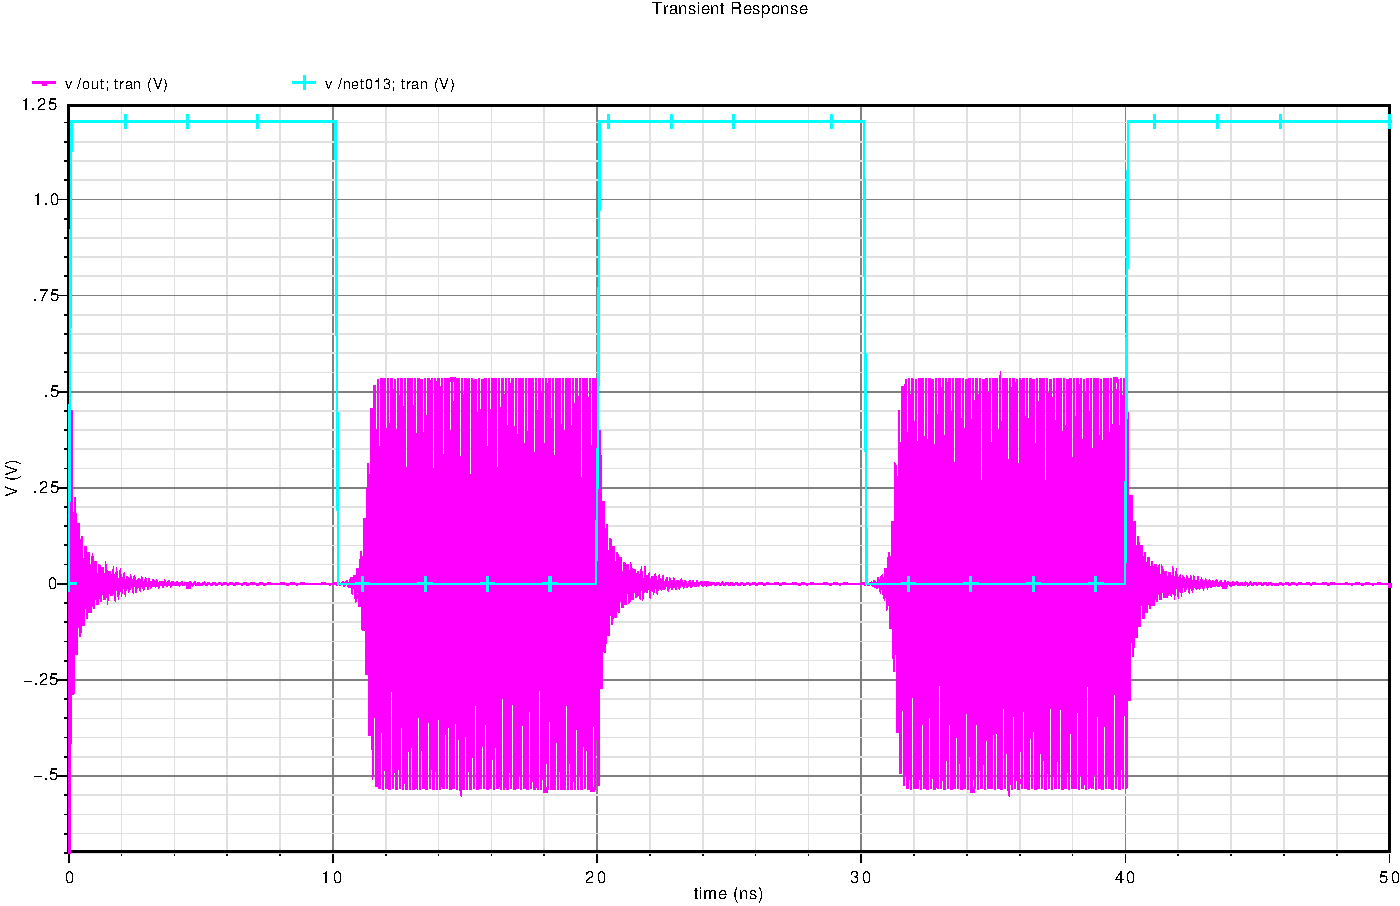
\includegraphics[width=\textwidth]{images/tipo2-impulsato.pdf}
\end{figure}
Oscillatore di Tipo 2, funzionamento impulsato.

\column[t]{0.25\textwidth}
	\vspace{0.5cm}
	\begin{figure}
	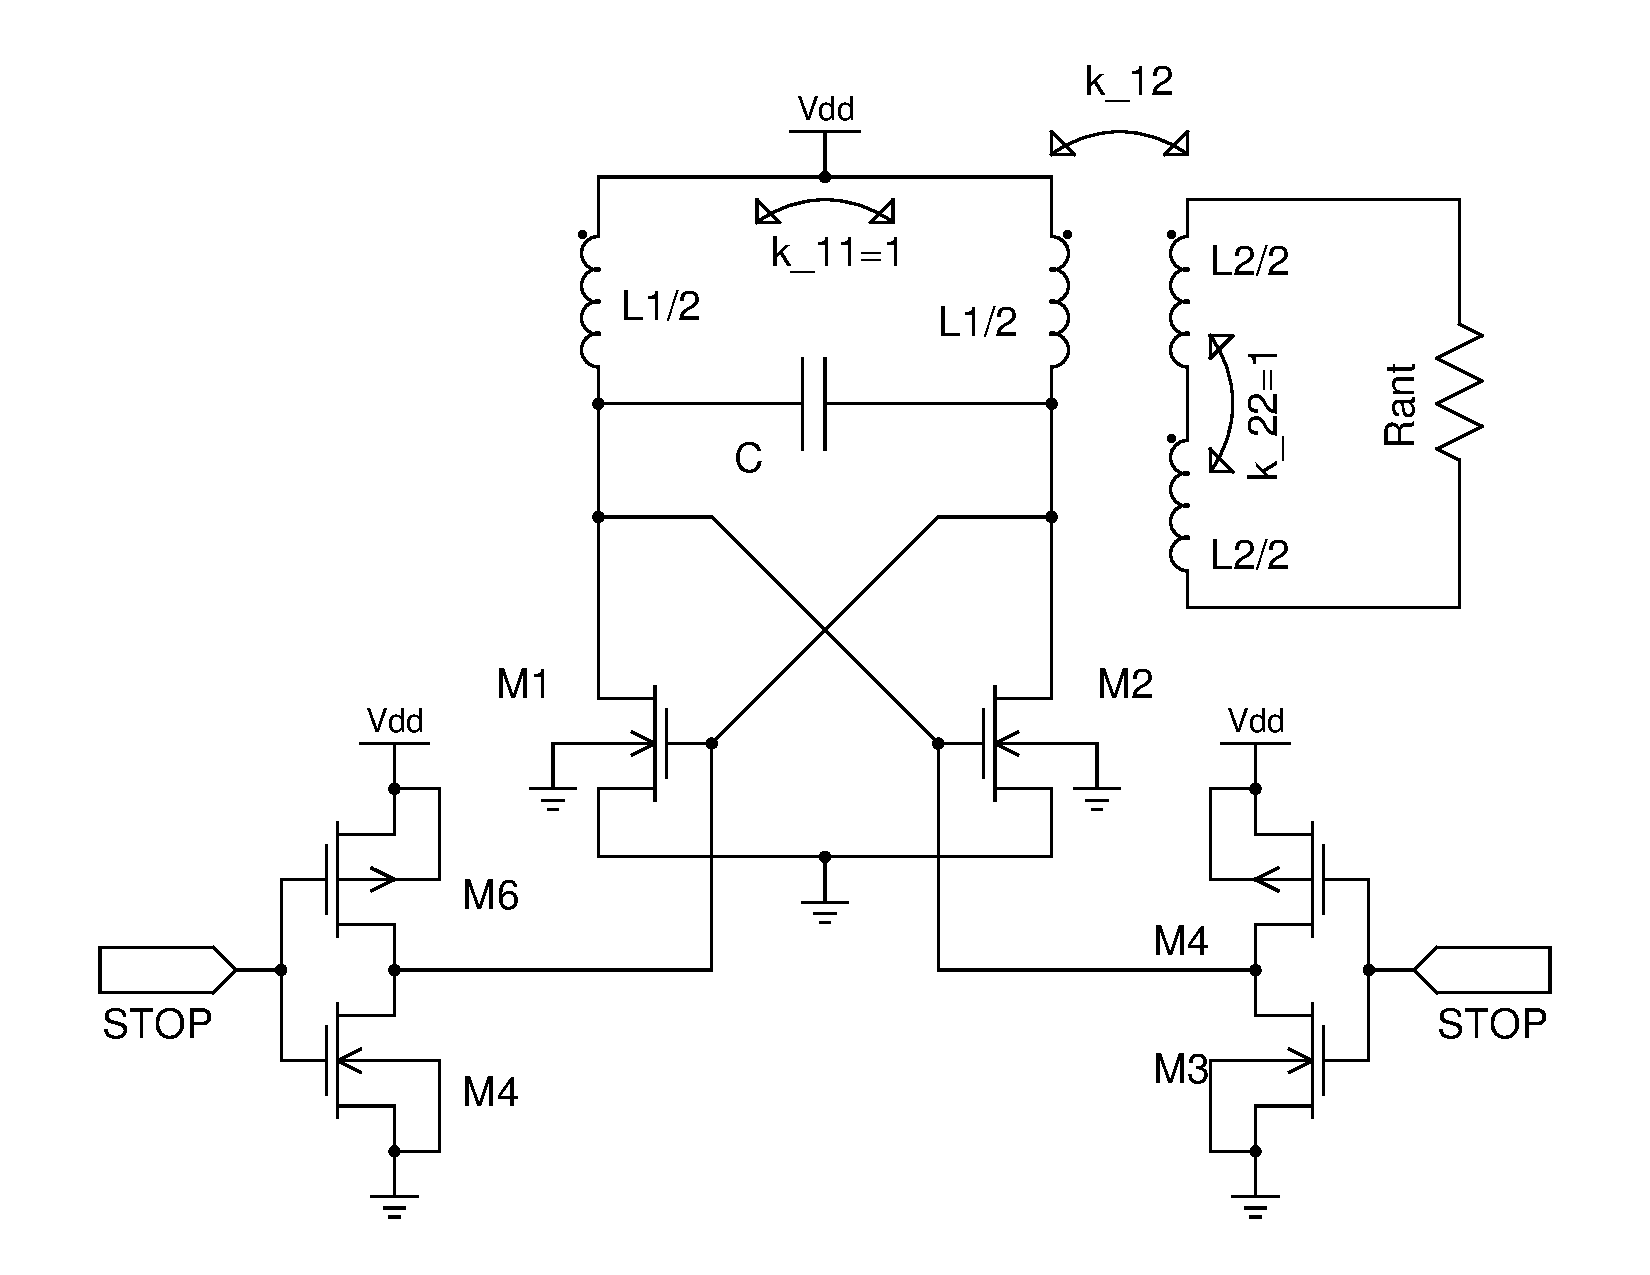
\includegraphics[width=1.3\textwidth]{images/tipo2.pdf}
	\end{figure}
\end{columns}
\end{frame}

\begin{frame}
\begin{itemize}
	\vfill
	\item Efficienza raggiunta:
	\begin{itemize}
		\item Tipo 1: $29,4\%$
		\item Tipo 2: $28,1\%$
	\end{itemize}
	\vfill
	\item Funzionamento impulsato:
	\begin{itemize}
		\item Accensione e spegnimento non istantanei 
		\item Tipo 1: ritardi marginalmente controllabili
		\item Tipo 2: più rapido, migliore controllo sull'inviluppo
	\end{itemize}
	\vfill
\end{itemize}
\end{frame}
%
%% Conclusion
\begin{frame}
\frametitle{Conclusioni}
\begin{itemize}
	\vfill
      \item Differenza trascurabile tra l'efficienza delle due tipologie
      \vfill
      \item Oltre all'efficienza, devono essere considerati:
	\begin{itemize}
            \item Area occupata dal circuito
            \item Consumo dinamico di potenza
      	\item Tempi di accensione e spegnimento
      \end{itemize}
      \vfill
	\item Sviluppi futuri:
	\begin{itemize}
		\item Approfondimento degli effetti dovuti all'inviluppo
		\item Valutazione del \emph{layout} del circuito
		\item Aumentare l'accuratezza del modello del trasformatore
	\end{itemize}
	\vfill
\end{itemize}
\end{frame}
\end{document}
